\documentclass{llncs}

\usepackage{url}
\usepackage{graphicx}
\usepackage{listings}
\usepackage{verbatim}
\usepackage[lined,linesnumbered,algochapter]{algorithm2e}
\usepackage{tikz}
\usetikzlibrary{arrows,automata}
\usepackage{xspace}
\usepackage{todonotes}          % Package for working draft comments
\usepackage{hyperref}           % Package for hyperlink references in the document


\usepackage[english]{babel}

\setcounter{secnumdepth}{2}
\setcounter{tocdepth}{3}

% define custom macros for specific formats or names
\newcommand{\uml}[1]{\texttt{#1}}
\newcommand{\cd}{\textsf{Class Diagram}}

%Colors for general listings
\definecolor{mygreen}{rgb}{0,0.6,0}
\definecolor{mygray}{rgb}{0.5,0.5,0.5}
\definecolor{mymauve}{rgb}{0.58,0,0.82}
%Colors for JSON listings
\colorlet{punct}{red!60!black}
\definecolor{background}{HTML}{EEEEEE}
\definecolor{delim}{RGB}{20,105,176}
\colorlet{numb}{magenta!60!black}

\lstset{ %
   backgroundcolor=\color{background},   % choose the background color; you must add \usepackage{color} or \usepackage{xcolor}
   basicstyle=\small\ttfamily,        % the size of the fonts that are used for the code
%   breakatwhitespace=false,         % sets if automatic breaks should only happen at whitespace
%   breaklines=true,                 % sets automatic line breaking
%   captionpos=b,                    % sets the caption-position to bottom
  commentstyle=\color{mygreen},    % comment style
%   deletekeywords={...},            % if you want to delete keywords from the given language
%   escapeinside={\%*}{*)},          % if you want to add LaTeX within your code
%   extendedchars=true,              % lets you use non-ASCII characters; for 8-bits encodings only, does not work with UTF-8
   frame=lines,                    % adds a frame around the code
%   keepspaces=true,                 % keeps spaces in text, useful for keeping indentation of code (possibly needs columns=flexible)
  columns=fixed,
  keywordstyle=\color{blue},       % keyword style
   language=Java,                 % the language of the code
%   morekeywords={*,...},            % if you want to add more keywords to the set
  numbers=left,                    % where to put the line-numbers; possible values are (none, left, right)
  numbersep=5pt,                   % how far the line-numbers are from the code
  numberstyle=\scriptsize\color{mygray}, % the style that is used for the line-numbers
%   rulecolor=\color{black},         % if not set, the frame-color may be changed on line-breaks within not-black text (e.g. comments (green here))
 showspaces=false,                % show spaces everywhere adding particular underscores; it overrides 'showstringspaces'
 showstringspaces=false,          % underline spaces within strings only
 showtabs=false,                  % show tabs within strings adding particular underscores
%   stepnumber=2,                    % the step between two line-numbers. If it is 1, each line will be numbered
  stringstyle=\color{mymauve},     % string literal style
  tabsize=2,                       % sets default tabsize to 2 spaces
%   title=\lstname                   % show the filename of files included with \lstinputlisting; also try caption instead of title
}


\begin{document}
\pagestyle{plain}
\pagenumbering{roman}

\title{fUML Refactoring with EMF}


\author{Sebastian Geiger (1127054) \and Kristof Meixner (9725208)}
\institute{Business Informatics Group\\Vienna Technical University}
\maketitle

\begin{abstract}
In this work we will present ideas and concepts for the refactoring of fUML models. The main contribution of this work is 
the extension of existing UML refactorings to cover not only the static aspect of UML such as class diagrams but to also 
include refactorings for dynamic
parts such as activity diagrams. In this work we will present basic concepts for refactoring of models with EMF and show how model semantics can be
preserved through the use of OCL constraints. In the remainder of the paper we then present our toolchain and the used technologies
of EMF (in particular Ecore and OCL) and how we used them for refactoring of models. We also present a discussion of EMF.Refactor, which shows how such refactorings
can be made available in the Eclipse GUIs such as the UML tree editor or Papyrus.
\end{abstract}

\tableofcontents
\newpage

\pagenumbering{arabic}

\section{Introduction}
% INTRODUCTION Models are getting more important in model-based software development, model-driven software development,
% model-driven architecture Models thus need to have a good quality

Model-based software development or model-driven software development is not only an extensive field of research but
receives also more and more attention from the industry. Nowadays models are not only used as visual explanations of
software concepts but as source for the development process itself. Thus models need to provide an abstraction of
the represented domains in a high quality. Mohagheghi et al. \cite{DBLP:journals/infsof/MohagheghiDN09} discussed possible 
quality attributes of models in their work.

% UML is a modelling language for models provided by the OMG that supports various types of models

To represent formal models the OMG developed UML \cite{man:UML} which by now advanced to an industry standard for 
modeling. With these common semantics enriched models can be preserved over time and even reused. Nevertheless models 
might have to be revised over the lifecycle of the software. With todays trend to more agile software 
development such as eXtreme Programming \cite{DBLP:journals/computer/Beck99} or Scrum \cite{DBLP:journals/software/RisingJ00} 
changes on models have to be even more efficient which brings refactoring of models into the focus of research.

% Refactoring is behavior preserving changing that should also improve quality

Refactoring is a technique that originates from source code development but can also be applied to model engineering.
The goal is to introduce behavior preserving changes \cite{mast:REFOOF} that increase the quality and understandability
of the models.

% Refactoring must preserve the behavior of all model types

While refactoring source code and textual code respectively applies to a single type of representation, in UML different
types of diagrams exist to represent various aspects of the models. This makes behavior preserving refactoring even harder 
as it needs to span over those different types of diagrams and semantics.

% Behaviour preservation can be tested statically or dynamically UML can be analysed statically fUML is a modelling
% language for models provided by the OMG that also allows execution and thus can be analysed dynamically

To prove the correctness of models before and after refactoring different approaches exist. One is the static analysis of
UML models via metrics and the attempt to find model smells \cite{DBLP:conf/models/ArendtTW13} which can be done via
OCL \cite{man:OCL}. Another way is to verify that models can be executed and to compare the execution traces of the 
original and refactored models. The OMG introduced a subset 
of UML named fUML \cite{man:FUML} which precisely defines semantics for class and activity diagrams to make them 
executable. 
Furthermore in \cite{DBLP:conf/icse/Mayerhofer12} Mayerhofer proposed a framework based on fUML that is able to execute
and debug those models.

% our approach is to combine both

The goal of this work is to introduce refactorings for fUML models, examine the requirements for co-refactoring of the
corresponding diagram types and define which co-changes have to be performed to preserve the behavior. Our approach to
verify
the correctness of the models after refactoring is twofold. On the one hand we use pre- and postconditions
\cite{rob99} to define if the specific changes can be applied and that the models are semantically correct afterwards.
On the other hand the models have to stay executable as well as traceable after the changes.

% we present a motivating example (class and activity diagrams) we provide some refactorings that target bothe diagram
% types we provide a how to test statically and dynamically, then refator and retest we provide a toolchain

% we provide some related work we provide a conclusion

The rest of the work is structured as follows. In section \ref{refactoring-examples} we give an overview over fUML and provide
a motivating
example of a model that is used throughout the paper. Section Y describes a selection of useful refactorings inspired by
Fowler \cite{fow99} and Markovic and Baar \cite{DBLP:journals/sosym/MarkovicB08} and their effects on class diagrams as
well as activity diagrams. In section \ref{sec:fuml-refactoring} we show which pre- and postcondition are needed for the refactorings and
how we refactor the models. In section \ref{sec:toolchain} we describe the toolchain that we use to define the models, 
implement a set of refactorings and test them. Related work is covered in section \ref{sec:relatedwork} and a conclusion is drawn in 
section \ref{sec:conclusion} to summarize the paper.

% what is refactoring and what does it mean in the context of models?
% what is fuml? what does fuml consist for diagram types?
% what is ocl? why do we use it and what for?

%fUML adds semantics to UML models that make it possible to create semantically closed models which can be executed on the model level. With
%fUML classic refactorings are not enough to refactor those models as they do not support the refactoring of the dynamic aspects of models
%such as activity diagrams.

\section{Motivation}
% what do we want to achieve?
fUML is an extension of UML which builds on a subset of UML classes with the purpose of adding semantics to UML models 
such that they can be executed on the model level. The dominant concept for this is the activity diagram. If a refactoring 
is performed on a UML model such as a class diagram, then any activity diagram which is releated to the class diagram, has 
to be checked and possibly changed as well. In section \ref{sec:fuml-refactoring} we will present some examples of fUML 
activity diagrams and present the implications \todo{so far we have not done that} that result from changing class 
diagrams (a procedure called co-refactoring).

Since a refactoring changes the structure of a model it is important to ensure that all changes maintain the original 
semantics of the model. Violating this requirement can result in models with either a different behavior, or in models 
which can no longer be executed. To ensure semantic preservation, two main techniques can be used. First, the refactoring 
can be broken down into smaller steps, each of which either guarantees to preserve the semantics of the model or makes it 
easier to verify that this is the case. Second, logical constraints can be used to limit refactorings on models to only 
those cases where semantic preservation can be ensured. For this purpose pre- and postconditions are specified with OCL 
constraints. A refactoring is then only applied if the original model satisfies the precondition before the refactoring is 
applied and the postcondition after the refactoring has been completed. Such constraints must be individually specified 
for each kind of refactoring that is to be performed. In this paper will introduce and discuss different OCL constraints 
for  the refactorings that we introduce.

Refactorings are only useful if they can be easily applied to the models through an easy to use process such as a 
graphical front end. EMF.Refactor allows the integration of refactorings into editors such as the UML tree editor or 
papyrus. It provides a Java API as well as a module concept to integrate refactorings. We will discuss the use of 
EMF.Refactor as part of our tool chain presentation.

% Why is it interesting to refactor models
% Why is it important in fUML that models remain consistent -> to preserve executability
% It is possible to use pre and post conditions in OCL to guarantee the semantic preservation of models during refactorings.

\section{Refactorings Examples}
\label{refactoring-examples}
% take model refactorings of markovic paper
% insurance example
% create example that supports all proposed refactorings

This section covers some general refactorings of UML class diagrams. As the basis of these refactorings an example from the insurance
domain is used. In the insurance business there are domain objects such as an insurance policy. Cars and trucks can be insured by 
adding them to the policy. There is an insurance company which has customers and employees and employees may purchase an insurance policy 
for one of their cars or trucks. Figure \ref{fig:classdiagramcomplex} shows a class diagram of such an insurance company. This class 
diagram would benefit from several possible refactorings such as an \textit{extract superclass} which can be applied to both \lstinline|Car| 
and \lstinline|Truck| to extract a \lstinline|Vehicle| class. A simple \textit{extract class} can be used on \lstinline|InsurancePolicy| to 
extract the \lstinline|from| and \lstinline|until| dates into their own \lstinline|InsurancePeriod\lstinline| class. As part of the 
\textit{extract superclass} refactoring two additional refactorings namely \textit{pull up attribute} and \textit{pull up method} are 
used to move the identical attributes and methods of both classes to the new superclass. As the 
attributes \lstinline|weight| and \lstinline|registration| are public, we can use \textit{encapsulate field} to make them private and 
provide getter and setter implementations. Finally the method addCar can be renamed into \lstinline|addVehicle| with \textit{rename method} 
and the \lstinline|addTruck| method can be removed with \textit{remove method}.

\begin{figure}[h!t]
 \centering
 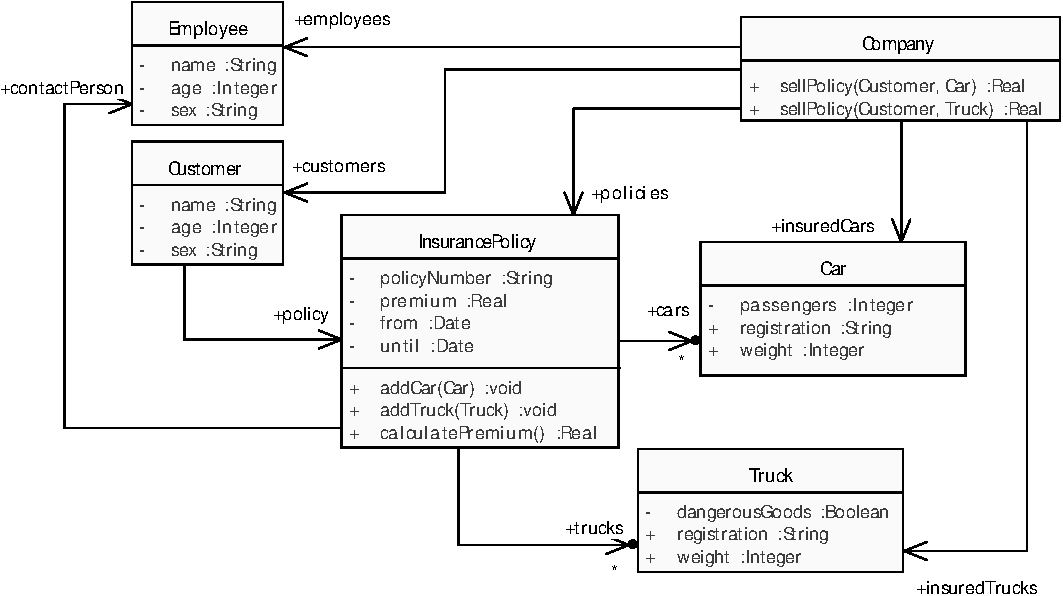
\includegraphics[scale=0.7]{images/ClassDiagramComplex.pdf}
 \caption{A car object that could benefit of extract class}
 \label{fig:classdiagramcomplex}
\end{figure}

For each of the methods in the \lstinline|InsurancePolicy| and \lstinline|Company| classes a separate activity diagram exists
which defines the semantics of these methods. As some of them are quite similar we will present only the diagrams for
addCar() in figure \ref{fig:addCar}, sellPolicy(Customer, Car) \ref{fig:sellPolicy} and calculatePremium() figure \ref{fig:calculatePremium}.


The activity for the \lstinline|addCar| operation is rather simple. It takes a car as a parameter and uses the
\lstinline|AddStructuralFeatureValueAction| to add the car to the insurance policy. In comparison \lstinline|calculatePremium| is
more complex, it calculates the insurance premium as follows:

\begin{itemize}
 \item Each insurance policy starts with a base fee of 50.
 \item For each car the number of passengers is multiplied by 5.
 \item The sum of multiplications for each car plus the base fee is the result.
\end{itemize}

\begin{figure}[h!t]
 \centering
 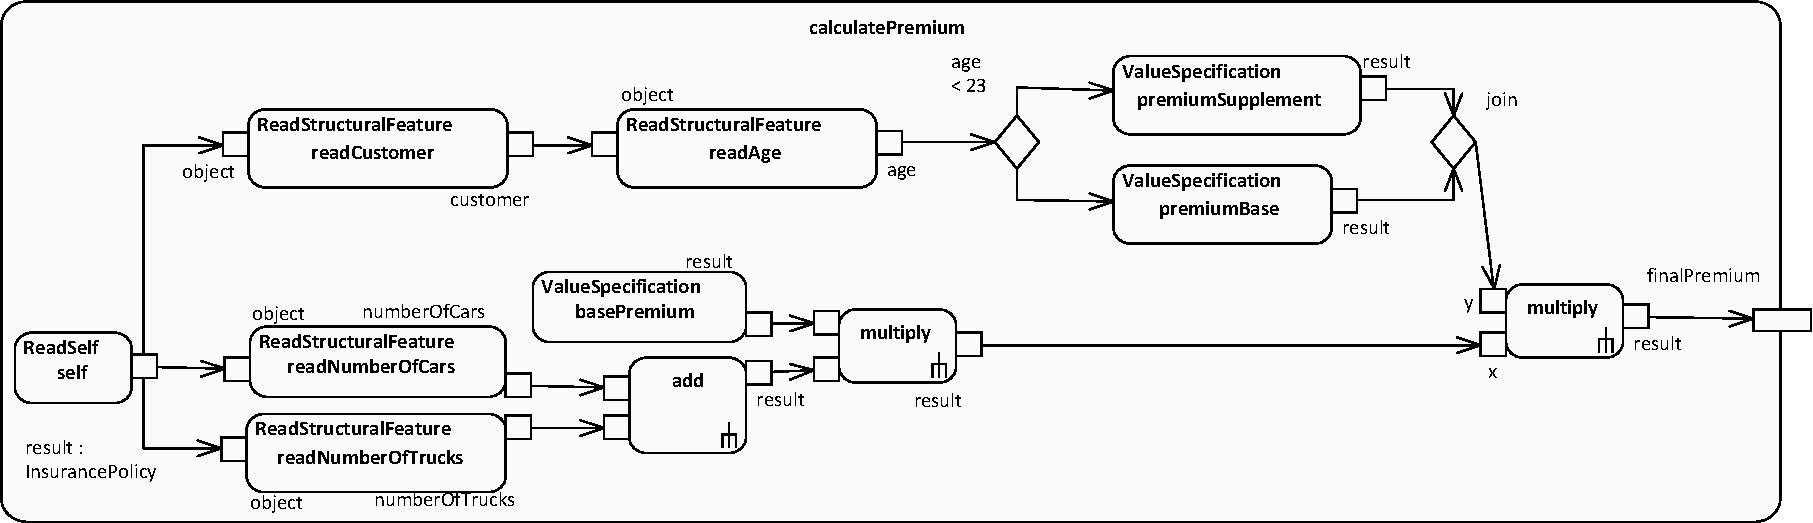
\includegraphics[scale=0.45]{images/calculatePremium.pdf}
 \caption{Activity diagram for calculate premium method}
 \label{fig:calculatePremium}
\end{figure}

\begin{figure}[ht]
 \centering
 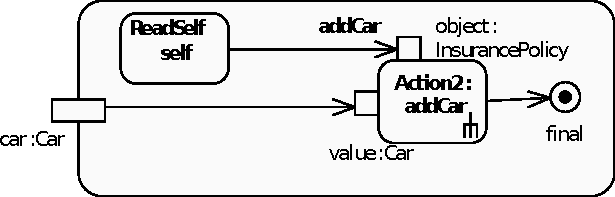
\includegraphics[scale=0.7]{images/addCar-activity_diagram}
 \caption{Add car activity diagram}
 \label{fig:addCar}
\end{figure}

\section{Refactoring of fUML models}
\label{sec:fuml-refactoring}
% abstract syntax of fUML and changes in diagrams
% ecore and ocl (with code examples)

In the last section we presented some models and their related activity diagrams. We also presented some of the possible 
refactorings such as \textit{extract superclass} or \textit{extract class}. This section discusses how the models actually 
need to be transformed in order to realize the refactoring.

Every model has two kinds of syntaxes. The concrete syntax, which defines how the model looks like, and the abstract
syntax, which defines the language elements and the grammar of the model. In order to refactor a model, we need to look at
its abstract syntax and transform it according to the refactoring rules.

A refactoring takes several parameters to configure the parts of the model that change and how they change. For example
the \textit{extract superclass} refactoring takes two parameters, the new name of the extracted superclass as well as
the list of classes that participate in the refactoring and which will receive the new class as their superclass.

In terms of the abstract syntax of these models, the two classes Car and Truck are instances of type class of the meta-model a 
superclass named Vehicle would be an instance of type Class as well, and can be associated with these two classes through the 
recursive attribute \textit{superclass} of the class \textit{Class} to create the inheritance hierarchy. In order to guarantee 
that the refactoring is possible, we must ensure that each class that participates in the 
refactoring does not already have a superclass.

\begin{figure}[h!t]
 \centering
 \begin{tabular}[]{l}
  \hline
  Extract class\\
  Extract superclass\\
  Rename Class\\
  Rename Method\\
  Rename Variable\\
  Add / Remove Parameter\\
  Encapsulate Field\\
  Pull up attribute\\
  Pull up operation\\
  Pull up association end\\
  Remove unused class\\
  \hline
 \end{tabular}
 \caption{Refactoring examples}
 \label{fig:refactoringlist}
\end{figure}

In this section\todo{Seems to be a misplaced section} we will present some general refactorings such as the ``extract superclass'' 
refactoring. A list of example refactorings is presented in figure \ref{fig:refactoringlist}.

\section{Toolchain and implementation}
\label{sec:toolchain}
For our toolchain we have relied on the moliz\footnote{http://www.modelexecution.org} repository, mainly for the ability to execute the fUML 
models in a virtual machine. The models are stored in XMI format and loaded with an EMF ResourceSet. The ResourceSet
can be used to retrieve a Resource object through an URI, which is then used to access the different objects in the model 
(see figure \ref{lst:resourceset}). All elements contained in the model are instances of Ecore (the implementation of
the MOF meta-meta-model) and they represent classes of the UML meta-model, which is implemented with Ecore.

\begin{figure}
 \begin{lstlisting}
resourceSet = new ResourceSetImpl();
resourceSet.getPackageRegistry().put(UMLPackage.eNS_URI,
                                     UMLPackage.eINSTANCE);
resourceSet.getResourceFactoryRegistry()
    .getExtensionToFactoryMap()
    .put(UMLResource.FILE_EXTENSION,
         UMLResource.Factory.INSTANCE);
File file = new File(umlModelFile);
URI uri = URI.createFileURI(file.getAbsolutePath());
    resource = resourceSet.getResource(uri, true);
 \end{lstlisting}
 \caption{Loading a UML model into a resource set}.
 \label{lst:resourceset}
\end{figure}

The extract superclass pre- and postconditions are shown in figure for single and multiple inheritance respectively.
\ref{lst:oclsuperclass}.

\begin{figure}[h!t]
 \begin{lstlisting}
Single Inheritance:
    pre: self.superClass->isEmpty() and 
         self.owner.ownedElement
            ->select(class|class.oclIsTypeOf(Class))
            .oclAsType(Class).name
            ->forAll(o | o<>newSuperClass.name)
    post: self.superClass->size() = 1

Multiple Inheritance:
   pre: self.owner.ownedElement
            ->select(class|class.oclIsTypeOf(Class))
            .oclAsType(Class).name
            ->forAll(o | o<>newSuperClass.name)
   post: self.general->contains(superClass)
 \end{lstlisting}
 \caption{OCL pre and post conditions for extract superclass}
 \label{lst:oclsuperclass}
\end{figure}

These ocl constraints are checked by the refactoring for each class object that participates
in the refactoring. An object to type OCL from the org.eclipse.ocl package is used to create and evaluate these queries
as can be seen in figure \ref{lst:ocl}.

\begin{figure}
\begin{lstlisting}
variable = ExpressionsFactory.eINSTANCE.createVariable();
variable.setName("newSuperClass");
variable.setType(UMLPackage.Literals.CLASSIFIER);
ocl.getEnvironment().addElement(variable.getName(),
                                variable, true);
query = helper.createQuery(
    "self.general->includes(newSuperClass)");
eval = ocl.createQuery(query);
eval.getEvaluationEnvironment()
    .add("newSuperClass", superClass);
if (!eval.check(clazz))
    return false;
\end{lstlisting}
\caption{OCL validation in Java}
\label{lst:ocl}
\end{figure}


% usage of fUML reference implementation of BIG
% how to load models?
% how to execute models?
% how to apply queries and changes?

\subsection{Model refactoring}
Describe our toolchain, how we created models, how we load them, what information of the abstract syntax we use for refactoring, etc.

\subsection{GUI Integration}
At the time of this writing our GUI integration is not finished, so we cannot describe it here. The idea is to use EMF.Refactor to add 

\section{Current Limitations}
Our work currently has several limitations. So far we have designed a set of related class and activity diagrams,
which are the basis for our refactorings. We have discussed the \textit{extract superclass} refactoring including its
pre- and post conditions and shown how it can be refactored with our toolchain. Until the final version of this
paper we will add several more refactorings from the list shown in figure \ref{fig:refactoringlist}, such as the
\textit{extract class}, the \textit{rename method}, the \textit{pullup method}, the \textit{pullup field} and 
\textit{rename variable} refactorings.

We have also briefly mentioned EMF.Refactor and we plan to extend out toolchain such that our implmented refactorings
can be invoked from the Eclipse GUI. At least we want to show that this is possible with our toolchain for at least one refactoring.

\section{Related Work}
\label{sec:relatedwork}
% Refactoring of prgram code

In this section we give an overview on the related work. Refactoring in a general way with preconditions was described
by Opdyke \cite{mast:REFOOF} in his master thesis and stated more precisely by Roberts \cite{rob99} who also introduced
postconditions for refactorings. Fowler \cite{fow99} generated an extensive yet simple to understand catalog of
refactorings for Java and Ruby which can be be adapted to model refactorings.

% Refactoring of models and OCL Code analysis via OCL

Suny{\'e} et. al. \cite{DBLP:conf/uml/SunyePTJ01} described how several refactorings can be applied to \textit{UML}
diagrams and introduced OCL as a possiblity to specify pre- and postconditions. Gorp et al. \cite{gorp03} extends the
discussion with the usage of \textit{OCL} for additional analysis such as code smells of models.

% Code execution via fUML

Despite of the further discussion of model refactoring (\cite{DBLP:conf/uml/CorreaW04}, \cite{DBLP:conf/ershov/BaarM06},
\cite{DBLP:journals/ase/ArendtT13}) most authors concentrate on static analysis and class diagram representations of
models. Dynamic analysis of models by execution and debugging \textit{fUML} models is discussed by Mayerhofer
\cite{DBLP:conf/icse/Mayerhofer12} and provides the basis for the approach discussed here. Mayerhofer et al.
\cite{DBLP:conf/models/MayerhoferLK12} furthermore introduce a runtime model and an
implementation\footnote{http://www.modelexecution.org} that is capable to test the models and directly show impacts of
refactorings.

% Refactoring implementation with EMF Refactor

Arendt and Taentzer \cite{DBLP:journals/ase/ArendtT13} present a framework that is based on \textit{Eclipse} and the
\textit{Eclipse Modelling Framework} which allows static model analysis and refactorings that are implemented in
different languages (Java, OCL \& Henshin) and can be directly extended in \textit{Eclipse}.


\section{Conclusion}
\label{sec:conclusion}
Refactoring models is a rather difficult task and it requires a concise knowledge of the involved technologies, with
the list of involved technologies being rather long. For one a reasonably well understanding of fUML is required, in
particular how class diagrams and activity diagrams are constructed and how they are related. It is not enough to simply
be able to draw both class and activity diagrams, as one also needs a good understanding of the meta-meta-model (MOF) and
the fUML and UML meta-model implementations in Ecore in order to understand and manipulate the model on the level of its 
abstract syntax. Finally an understanding of EMF (in particular Ecore and OCL) is required. While MOF and OCL are both 
modeling concepts and languages respectively, EMF contains implementations for them in Java with a complex API. 
Understanding these APIs of Ecore and OCL is required to perform the refactorings and was a prerequisite to build
our toolchain.

With the toolchain in place another challenge was to identify the required steps to perform the actual refactoring work.
In particular this meant to identify how the activity diagrams need to change if a change is made in the class
diagram.

Most of our efforts in the development of this work were focused on gaining a comprehensive understanding of the
technologies described above, to develop the tool chain and to draw the various diagrams presented in this paper and make 
them executable. We have presented a comprehensive set of diagrams as the basis for our refactoring work and demonstrated 
the feasibility of our tool chain. However a more comprehensive evaluation of the different refactorings including the 
specification of pre- and postconditions OCL in is still required and will be the focus of our ongoing efforts.

\newpage
\bibliographystyle{acm}
\bibliography{references}

\end{document}
